
\documentclass{article} 
\usepackage{iclr2026_conference,times}

\input{math_commands.tex}

\usepackage{hyperref}
\usepackage{url}
\usepackage{graphicx}

\title{Formatting Instructions for ICLR 2026 \\ Conference Submissions}


\newcommand{\fix}{\marginpar{FIX}}
\newcommand{\new}{\marginpar{NEW}}

\begin{document}

\maketitle

\begin{abstract}
We find that model conviction in an answer is not reached through gradual accumulation, but through a ``confidence leap'': a sudden and sharp increase in its probability. Using this signal, we introduce a training‑free, model‑agnostic early‑stopping rule based on the rapid increase in answer probability; across experiments, it reduces generation without sacrificing accuracy and often improves it. 

\end{abstract}

\section{Introduction}
\label{sec:introduction}

Large reasoning models often generate long chain-of-thought (CoT) traces before emitting a final answer. A common assumption is that confidence in the correct answer grows gradually as evidence accrues. In this work, we show that, for multiple-choice QA, confidence typically changes \emph{non-monotonically} and decisive commitments are made via a sudden ``confidence leap''—a sharp jump in the probability of one option between consecutive reasoning chunks.

We operationalize this observation by segmenting CoT traces into semantically coherent chunks and probing the model’s answer distribution after each chunk by temporarily closing the reasoning phase. Two robust empirical regularities emerge: (i) across tasks, examples cluster by the number of answer switches (0, 1, or $>1$); and (ii) among instances with exactly one switch, the probability of the ultimately correct answer exhibits a large positive jump precisely at the \emph{critical chunk}—the point where the model changes its mind for the last time.

Motivated by these findings, we propose a simple, training-free, model-agnostic early-stopping heuristic: stop generation the first time any answer option’s probability increases by more than a threshold relative to the previous chunk, and return the currently most probable option. This rule yields substantial savings in generated content while maintaining—and often \emph{increasing}—overall accuracy.

Our contributions are threefold:

- \textbf{Phenomenology of switching:} We characterize how accuracy depends on the number of answer switches within a CoT trace and document that 1-switch cases are both common and high-accuracy when stopped at the commitment point.
- \textbf{Confidence leap at the critical chunk:} We show that the probability of the correct option jumps sharply at the last switch, whereas jumps toward an incorrect option are smaller and rarer.
- \textbf{A practical early-stopping rule:} We introduce a probability-jump heuristic that is training-free and model-agnostic, achieving strong accuracy with significant chunk/token savings and transferring across models: feeding another model the source model’s reasoning up to its critical chunk boosts the second model’s accuracy.

\section{Related Work}
\label{sec:related_work}

...

\section{Data Collection}
\label{sec:data_collection}
The long Chain-of-Thought (CoT) outputs from reasoning models often contain multiple intermediate steps and shifts in reasoning. We aim to explore whether the dynamics of the model's confidence can be tracked throughout this process. This section describes how we segment reasoning traces into meaningful units, obtain confidence measurements at each step, and details our overall experimental setup.

We focus on the multiple-choice question answering (MCQA) format as it provides a constrained output space (e.g., options A, B, C, D), allowing for a direct and unambiguous measurement of the model's confidence distribution over potential answers.

First, the reasoning trace for each problem, encapsulated within \texttt{<think>} tokens, is extracted. The trace is then split into paragraphs using ``\verb|\n\n|'' as a delimiter. We identify the start of a new reasoning path by detecting semantic keywords that signal a shift in thought, such as ``wait'', ``alternatively'', and ``hmm''. A complete list of keywords is provided in Appendix~\ref{app:keywords}. Paragraphs belonging to the same reasoning path are then merged to form a single semantic unit, which we define as a \textit{chunk}.

After each reasoning chunk, we measure the model's confidence in each of the potential answers $\{A, B, C, D\}$ by actively querying its conclusive answer guess at that stage. Specifically, for each chunk $i$, we construct a prompt containing the original question followed by the reasoning trace up to and including that chunk. We then append the closing \texttt{</think>} tag, which signals the model to terminate its reasoning and generate a final answer. The model's confidence is then defined as the softmax-normalized probability distribution over the answer tokens \{`A', `B', `C', `D'\} at this specific, post-reasoning position. This procedure provides a snapshot of the model's belief state as if it were forced to conclude its reasoning at the end of each chunk.

\section{Empirical Characterization of Switching and Confidence Leaps}
\label{sec:phenomena}

\subsection{Switching patterns vs. accuracy}
We group examples by their number of answer switches (0, 1, 2, 3+). Figure~\ref{fig:stacked_accuracy_changes} shows accuracy as a function of reasoning length, with bars stacked by switch count. Two trends are salient: (i) longer traces exhibit more switching; (ii) conditioning on switch count, 1-switch cases maintain relatively high accuracy compared to $>1$ switches.

\begin{figure}[t]
    \centering
    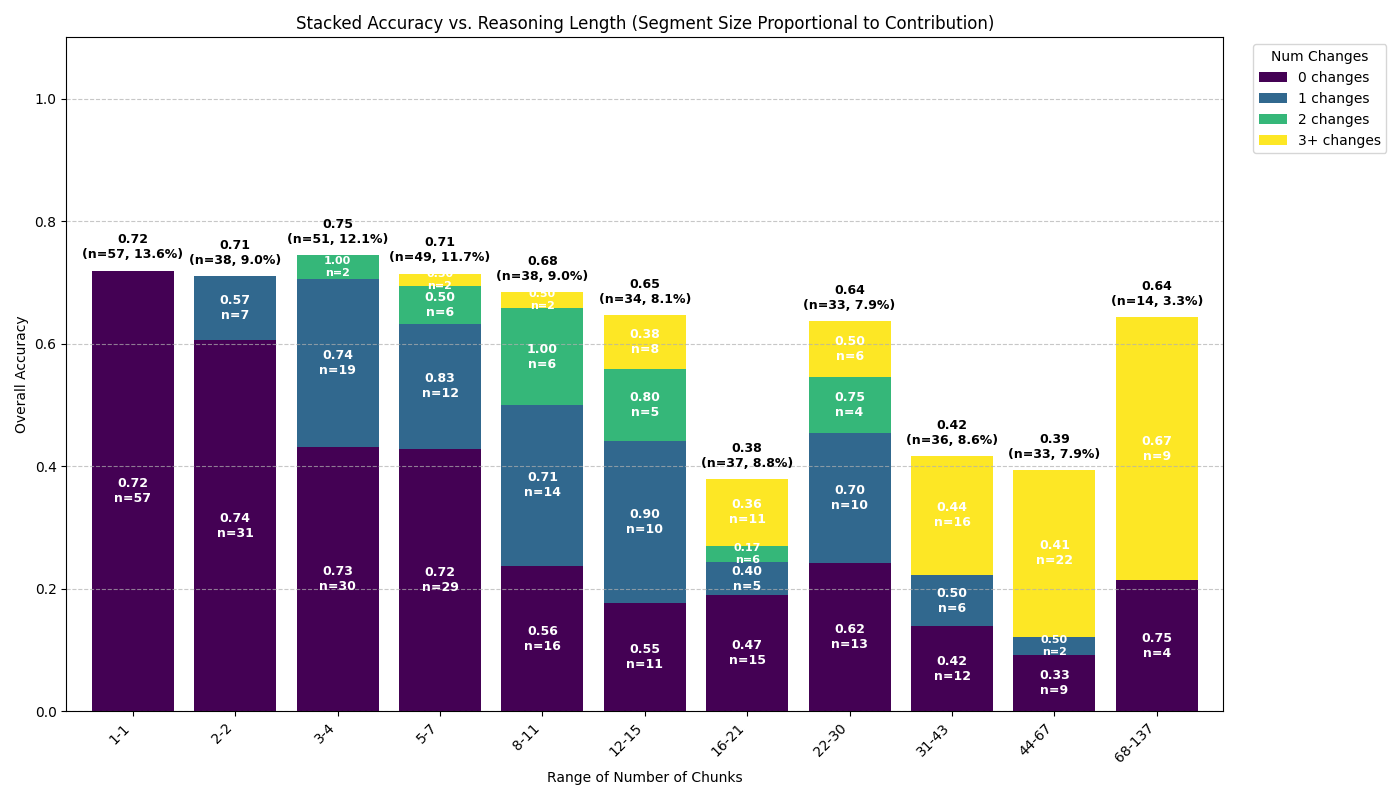
\includegraphics[width=0.95\linewidth]{analysis_results/accuracy_vs_length/binned_accuracy_vs_length_by_changes_reasoning_traces_gpqa_Qwen_Qwen3-32B.png}
    \caption{Stacked accuracy vs. reasoning length on GPQA, with segments indicating the proportion and accuracy of traces stratified by number of answer switches (0, 1, 2, 3+).}
    \label{fig:stacked_accuracy_changes}
\end{figure}

% Inserted: table of accuracy by number of switches (0,1,2,3,>4)
\begin{table}[t]
    \centering
    \caption{Accuracy and counts by number of switches (GPQA). Buckets are 0, 1, 2, 3, and $>4$. Cases with exactly 4 switches: $n=15$, accuracy $=0.333$.}
    \label{tab:acc_by_switches}
    \begin{tabular}{lcc}
    \hline
    Switches & Accuracy & Count \\
    \hline
    0  & 0.652 & 227 \\
    1  & 0.698 &  86 \\
    2  & 0.613 &  31 \\
    3  & 0.500 &  18 \\
    $>4$ & 0.465 &  43 \\
    \hline
    \end{tabular}
\end{table}

\subsection{The critical chunk exhibits a confidence leap}
Restricting to 1-switch traces, let $k$ be the first (and last) index where the model’s top answer changes. Comparing the probability of the ground-truth option at chunk $k$ versus $k{-}1$ reveals a large positive jump at $k$ when the switch is \emph{to} the correct option, and a markedly smaller (often negative) change when switching \emph{from} correct. Figure~\ref{fig:prob_change_scatter} visualizes the before/after probabilities at the critical chunk.

\begin{figure}[t]
    \centering
    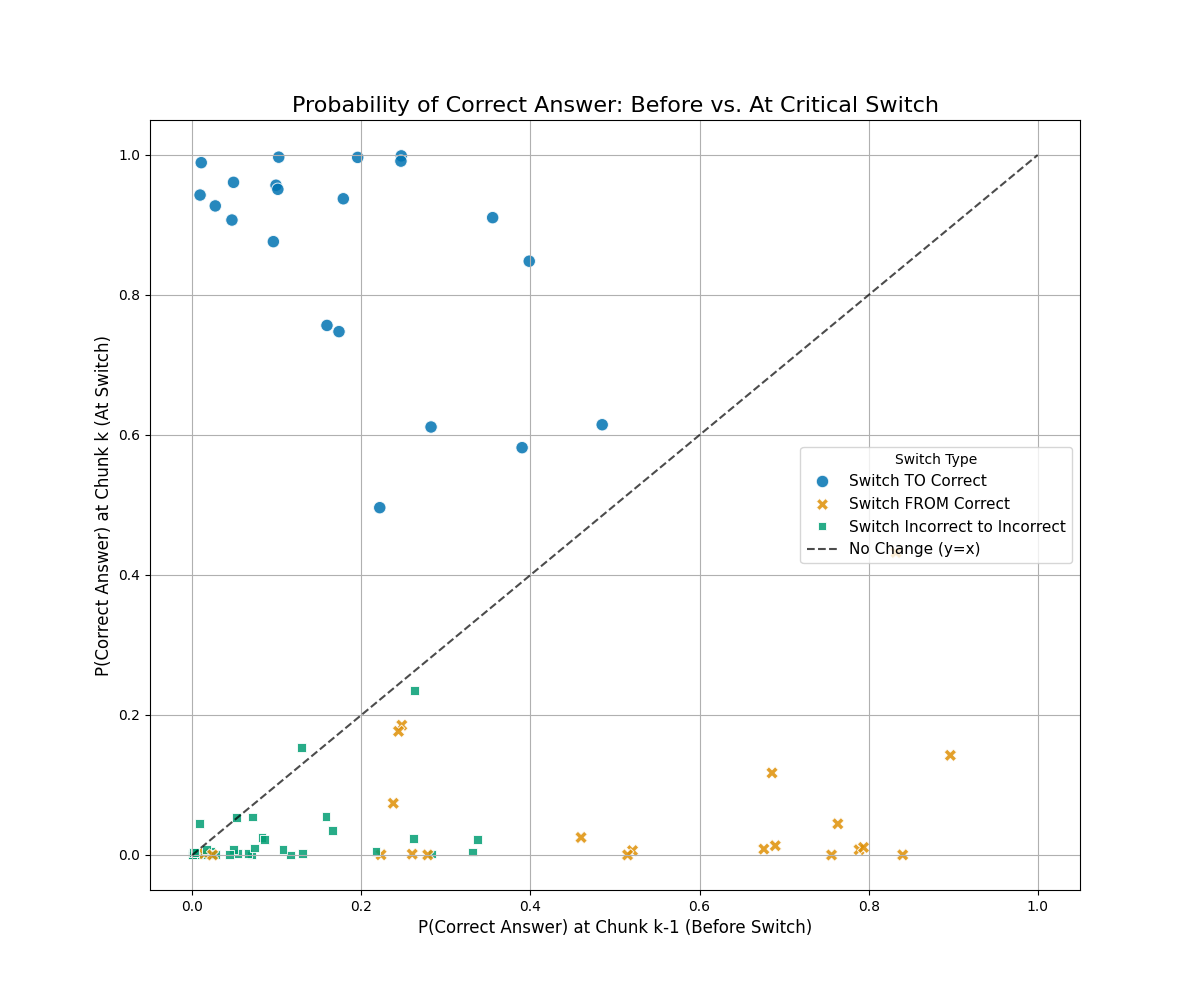
\includegraphics[width=0.75\linewidth]{analysis_results/critical_chunk_prob_change/prob_change_scatter_reasoning_traces_gpqa_Qwen_Qwen3-32B.png}
    \caption{Probability of the correct option before (chunk $k{-}1$) vs. at (chunk $k$) the critical switch (1-switch traces). Points above the diagonal indicate an increase. The dominant pattern is a large upward jump when switching to the correct answer.}
    \label{fig:prob_change_scatter}
\end{figure}

\section{A Training-Free Early-Stopping Rule}
\label{sec:heuristic}

We stop generation at the first chunk $k$ where the increase in any option’s probability exceeds a threshold $\tau$: stop if $\max_{\ell \in \{A,B,C,D\}} \big( p_k(\ell) - p_{k-1}(\ell) \big) > \tau$, and output $\arg\max_{\ell} p_k(\ell)$. This requires no additional training and applies to any model exposing token probabilities after a forced stop.

On GPQA, sweeping $\tau$ yields a favorable trade-off (Figure~\ref{fig:tradeoff}). Around the best operating point, overall accuracy peaks while reducing average chunks/tokens generated. For example, we observe strong precision at trigger time, substantial coverage, and non-trivial overall token savings despite only stopping in a subset of cases.

\begin{figure}[t]
    \centering
    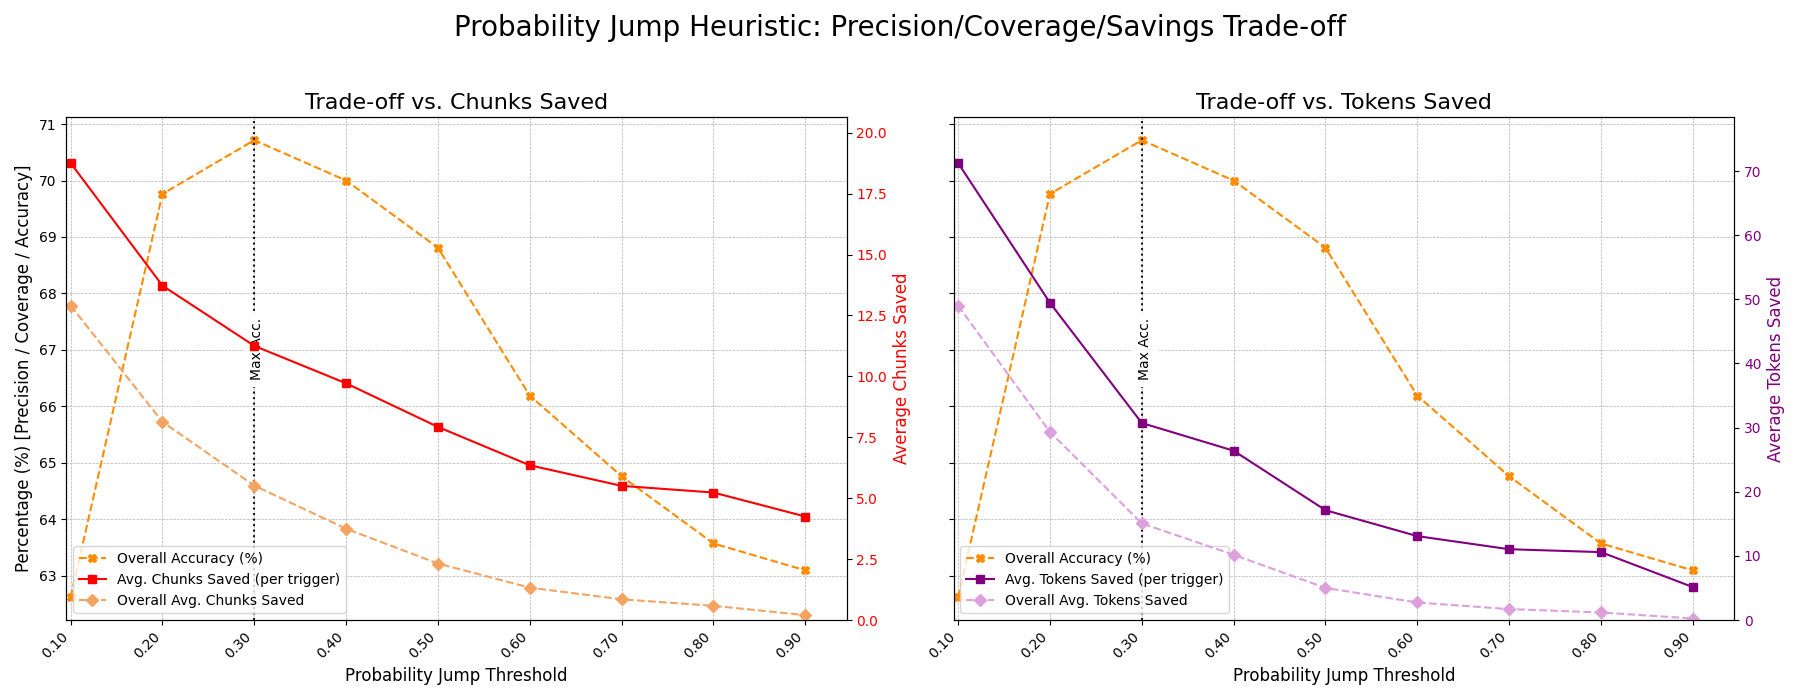
\includegraphics[width=0.95\linewidth]{analysis_results/jump_heuristic/jump_heuristic_tradeoff_reasoning_traces_gpqa_Qwen_Qwen3-32B.png}
    \caption{Probability-jump early stopping: sweep over threshold $\tau$ shows overall accuracy alongside chunk/token savings. Best operation attains competitive or improved accuracy with significant savings.}
    \label{fig:tradeoff}
\end{figure}

\paragraph{Transfer across models.} To test whether the signal is semantic rather than a compute-time artifact, we feed another model the source model’s reasoning prefix up to the critical chunk. The second model’s accuracy improves most when given the prefix through the critical chunk (vs. shorter prefixes), supporting the view that useful intermediate content is encoded in the \emph{text} of reasoning and transfers across models.

\appendix
\section{Chunking keywords}
\label{app:keywords}
We use a small, fixed list of keywords to detect semantic restarts and branch transitions when chunking CoT traces. The seed list includes: \textit{wait}, \textit{hmm}, \textit{hold on}, \textit{alternatively}, \textit{on second thought}, \textit{another approach}, \textit{re-evaluate}, \textit{correction}, \textit{let’s check}, \textit{consider}. We then merge adjacent paragraphs into a chunk until the next detected restart.

\bibliography{iclr2026_conference}
\bibliographystyle{iclr2026_conference}

\end{document}
